\section{Testing and Verification}

We performed 4 tests on our final design, 1 test to ensure our hardware works correctly, 1 test to verify our software, and 2 tests on the full work flow to confirm that the project is working as a whole.

\subsection{Hardware Test}

To test that our overlay tiles are working correctly, we built a single tile onto the Virtex 5 FPGA and connected the inputs and outputs of the tile to the switches and LEDs of the FPGA.
We then pushed in a manually composed bitstream through a serial connection to program the tile's function and routing.
Once the tile was programmed, we verified the behaviour of the tile against what we expected from the bitstream, including the functions in the lookup tables, and the routing of input and output signals.
The tile can be re-programmed as many times as we like to test different functions and signal routing.

Excerpt from our manually generated bitstream:
0FFFFFFFFFFFFFFFE
18000000000000000
0FFFFFFFFFFFFFFFF
08888888888888888

The above snippet programs the four 6-input lookup tables and their connected flops.
The leftmost value indicates whether or not the output of the lookup table is routed through a flop (0=no, 1=yes), and the rest determines the function of the lookup table itself.
From the top, the lookup tables are programmed as follows: 6-input OR gate, 6-input AND gate with flop, always 1, 2-input AND gate.

The test showed that our tile was fully functional, behaving as expected in both lookup table functionality and correct routing.
The test proved that our project satisfied the following requirements:
\begin{itemlist}
	\item H1: The tile was implemented on a Virtex 5 FPGA chip
	\item H3: The tile only needed to be built once on the chip, after which it was re-programmable via serial cable without the need to be re-flashed onto the chip.
	\item H4: The tile had connectivity to the switches and LEDs of the chip
	\item S2: Our bitstream sending/receiving software operated correctly in order to program the tile
	\item G1: The tile implemented four 6-input lookup tables
\end{itemlist}

\subsection{Software Test}

To test our bitstream generation software, we wrote simple circuits in verilog, then used our selected third-party software to synthesize, place and route the circuits according to our architecture.
We then took the resultant output and used our software to generate a bitstream capable of programming our overlay circuit.
We went through the generated bitstream manually to ensure the logic and routing matched the overlay, and that it was of the appropriate format for the overlay.
Because of the size of the bitstream, this test is restricted to simple circuits on a small overlay.

The bitstream passed manual inspection; it was structured correctly and the logic and routing matched the third-party software outputs.
The test proved that our project satisfied the following requirements:
\begin{itemlist}
	\item S1: The software was successful in translating VPR placement and route data into a bitstream appropriate for the overlay FPGA
\end{itemlist}

\subsection{Full Tool Flow Test}

Finally, to test the project as a whole, we combined the hardware and software tests, building test circuits in verilog, passing them through VPR and translating the output into a bitstream, and injecting the bitstream onto a full overlay on the Virtex 5 for testing.

We first tested the project with a simple buffer circuit, where inputs to the overlay were connected directly to outputs.
When the buffer proved successful, we moved on to a slightly more complex circuit, an 8-bit adder.

Verilog code for the adder:

\begin{tabular}{|p{7cm}|}
\hline
\begin{verbatim}
module test( in, out);

input  [7:0] in;
output [7:0] out;

assign out = in[7:4] + in[3:0];

endmodule
\end{verbatim}
\\ \hline
\end{tabular}

\begin{figure}[!h]
	\centering
	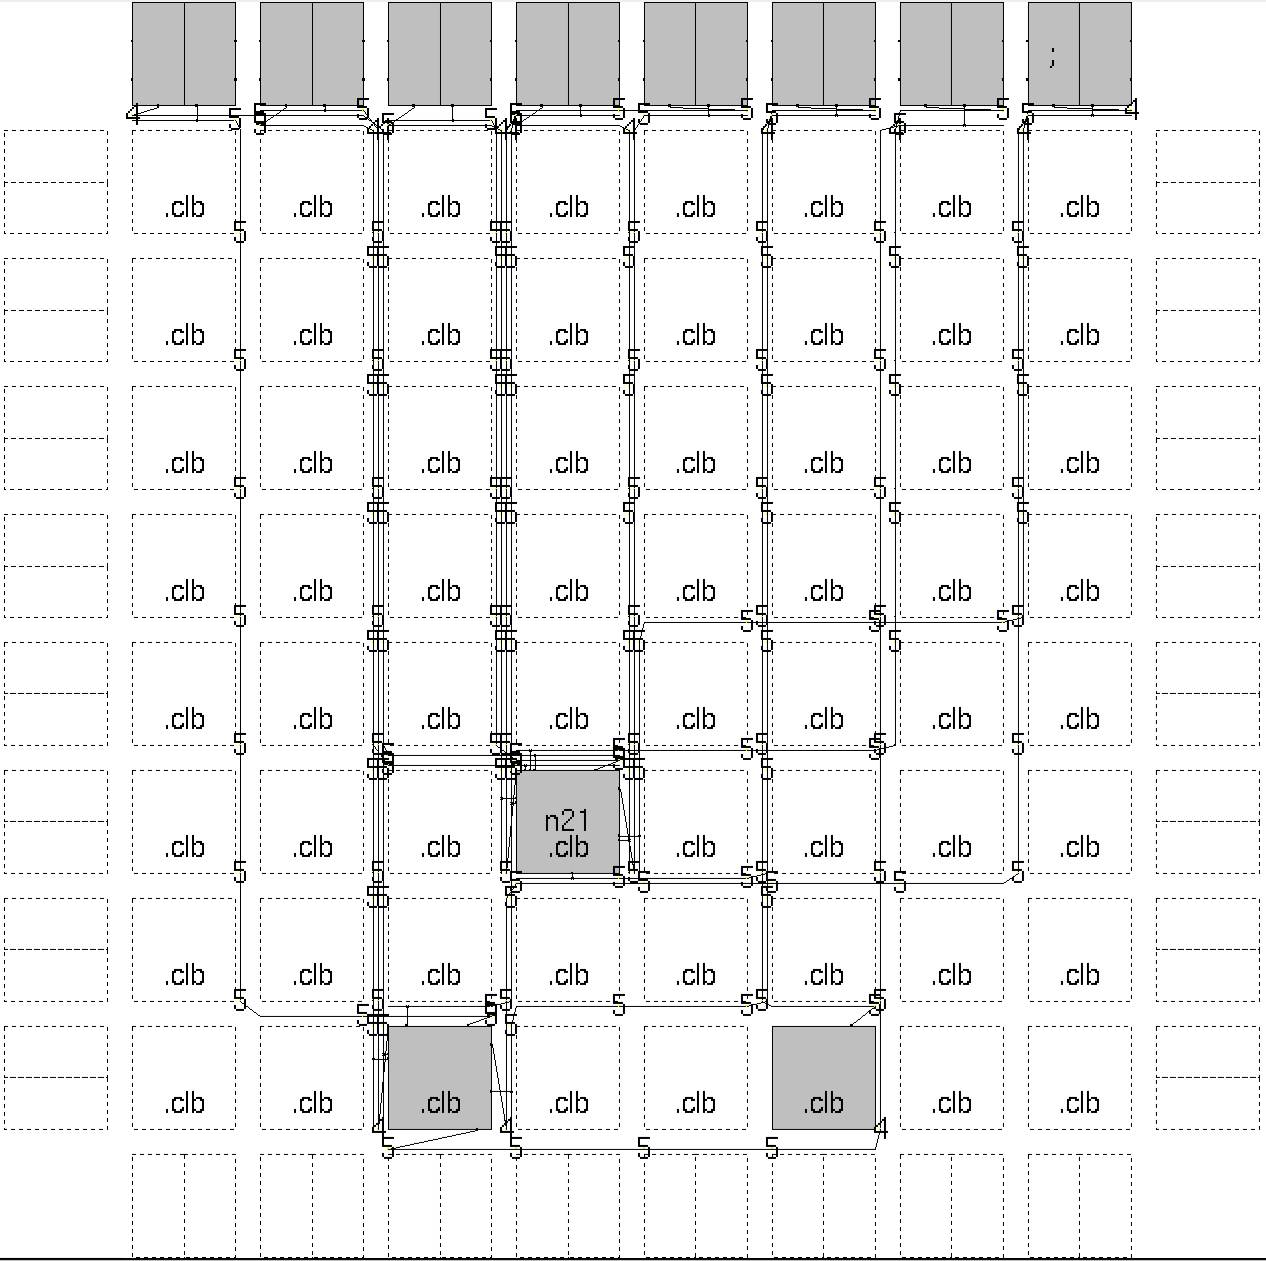
\includegraphics[scale=0.5]{vpr-adder.png}
	\caption{VPR screenshot of 8-bit adder placement and routing}
	\label{adder}
\end{figure}

\figref{adder} shows a screenshot of VPR after placing and routing the 8-bit adder.

Excerpt from VPR placement output:

\begin{tabular}{|p{13cm}|}
\hline
\begin{verbatim}
Netlist file: adder.net Architecture file: adder.arch.xml
Array size: 8 x 8 logic blocks

#block name x y subblk block number
#---------- -- -- ------ ------------
top^in~0 1 9 0 #0
top^in~1 2 9 0 #1
top^in~2 3 9 0 #2
top^in~3 4 9 0 #3
top^in~4 5 9 0 #4
top^in~5 6 9 0 #5
top^in~6 7 9 0 #6
top^in~7 8 9 0 #7
out:top^out~0 1 9 1 #8
out:top^out~1 2 9 1 #9
out:top^out~2 3 9 1 #10
out:top^out~3 4 9 1 #11
out:top^out~4 5 9 1 #12
out:top^out~5 6 9 1 #13
out:top^out~6 7 9 1 #14
out:top^out~7 8 9 1 #15
n21 4 3 0 #16
top^out~0 3 1 0 #17
top^out~5 6 1 0 #18
\end{verbatim}
\\ \hline
\end{tabular}

The above excerpt shows the locations in the overlay VPR has placed logic components and input/output pads.
This is one of the output files our software utilizes to generate the bitstream.

Excerpt from VPR routing output:

\begin{tabular}{|p{5cm}|}
\hline
\begin{verbatim}
Net 13 (top^out~6)

SOURCE (3,1) Class: 1
OPIN (3,1) Pin: 18
CHANX (3,0) Track: 0
CHANX (4,0) Track: 0
CHANX (5,0) Track: 0
CHANX (6,0) Track: 0
CHANY (6,1) Track: 0
CHANY (6,2) Track: 0
CHANY (6,3) Track: 0
CHANY (6,4) Track: 0
CHANY (6,5) Track: 0
CHANY (6,6) Track: 0
CHANY (6,7) Track: 0
CHANY (6,8) Track: 0
CHANX (7,8) Track: 0
IPIN (7,9) Pad: 3
SINK (7,9) Pad: 3
\end{verbatim}
\\ \hline
\end{tabular}

The above excerpt shows the routing done by VPR of one net in the overlay.
Each line traces the path of the signal as it moves through the overlay, starting at the source of the signal and ending at the sink.
This is part of another output file that our software uses to generate the bitstream.

The overlay functioned correctly with the adder, proving that our design meets the following requirements:
\begin{itemlist}
	\item H1: The overlay was implemented on a Virtex 5 FPGA chip
	\item H2: The overlay was customized to 8x8 tiles, with a bus width of 4, logic block input per side of 4, and 4 look up tables per logic block
	\item H3: The overlay only needed to be built once on the chip, after which it was re-programmable via serial cable without the need to be re-flashed onto the chip
	\item H4: The overlay had connectivity to the switches and LEDs of the chip
	\item S1: Our software generated the overlay bitstream by parsing and translating VPR placement and routing output files
	\item S2: Our bitstream sending/receiving software operated correctly in order to program the tile
	\item G1: The tile implemented four 6-input lookup tables
	\item G2: The 8x8 logic grid contains 256 overlay logic elements, well over 100
\end{itemlist}

% for each requirement #, report final result. comment on degree of compliance.
% can add more detailed comments after the table.

% refer to appendix b

% show evidence (vpr screenshots, etc)

